\chapter{Working Principle and Physics}
\label{ch:principle}

This chapter explains why a cube can balance on an edge or a corner by means of internal reaction
wheels. The equations are simplified models that explain the behaviour and the structure of the
controllers in \cref{ch:firmware}; the gains of the Cubilox Mk1 were tuned experimentally and not
derived from an identified model.

\section{The cube as an inverted pendulum}

A cube resting on one of its edges or corners is an \emph{inverted pendulum}: its centre of mass
lies above the pivot, and any small deviation from the upright position produces a gravitational
torque that increases the deviation. For a cube with edge length $a$ and its centre of mass in the
geometric centre, the distance between pivot and centre of mass is
\begin{equation}
  l_\text{edge} = \frac{a}{\sqrt{2}} \qquad\text{and}\qquad l_\text{vertex} = \frac{\sqrt{3}}{2}\,a .
\end{equation}
For the Cubilox Mk1 with $a = \SI{157}{mm}$, and assuming the centre of mass in the geometric
centre, this gives $l_\text{edge} \approx \SI{111}{mm}$ and $l_\text{vertex} \approx \SI{136}{mm}$.
In the balanced edge position the faces adjacent to the edge are inclined by \ang{45}; in the
balanced vertex position the space diagonal through the pivot corner is vertical, so each face
normal makes an angle of $\arccos(1/\sqrt{3}) \approx \ang{54.7}$ with the vertical.

\section{Reaction wheels}

A reaction wheel is a flywheel driven by a motor that is fixed to the body. When the motor applies
a torque $\tau$ to the wheel, the wheel applies the opposite torque $-\tau$ to the body
(Newton's third law). Accelerating a wheel therefore rotates the cube in the opposite direction,
without any contact to the ground other than the pivot. The torque is only available while the
wheel speed changes: a wheel spinning at constant speed produces no torque. Since the speed of a
real motor is limited, a wheel cannot be accelerated in the same direction forever. This leads to
the need for wheel speed feedback, explained in \cref{sec:wheel_speed}.

The reaction torque is proportional to the moment of inertia of the wheel and its angular
acceleration. A large moment of inertia with little mass is achieved by placing mass far from the
axis; this is why the wheels of the Cubilox Mk1 carry screws and nuts on their rim
(\cref{sec:wheels}).

\section{Balancing on an edge (one axis)}
\label{sec:edge_model}

On an edge, the cube can only rotate about the edge, and one reaction wheel whose axis is parallel
to that edge is sufficient. Let $\theta$ be the tilt angle measured from the balance point,
$\Theta$ the moment of inertia of the cube about the edge, $m$ its mass, $g$ the gravitational
acceleration, $\Theta_w$ the moment of inertia of the wheel and $\omega_w$ the speed of the wheel
relative to the body. A simplified planar model is
\begin{align}
  \Theta\,\ddot\theta &= m g\, l_\text{edge} \sin\theta - \tau, \label{eq:edge_body}\\
  \Theta_w \left(\dot\omega_w + \ddot\theta\right) &= \tau, \label{eq:edge_wheel}
\end{align}
where $\tau$ is the motor torque acting on the wheel. Linearised around $\theta = 0$
($\sin\theta \approx \theta$), the uncontrolled system has a real positive eigenvalue
$\lambda = \sqrt{m g\, l_\text{edge}/\Theta}$: without control, a small deviation grows
exponentially and the cube falls.

A linear state feedback of the tilt angle, the tilt rate and the wheel speed stabilises the
system:
\begin{equation}
  u = K_1\,\theta + K_2\,\dot\theta + K_3\,\omega_w ,
  \label{eq:edge_law}
\end{equation}
where $u$ is the motor command. In the firmware, these three terms are the gains
\cmd{ek1}, \cmd{ek2} and \cmd{ek3} (\cref{sec:edge_controller}):
\begin{itemize}
  \item the \textbf{angle term} $K_1\theta$ pushes the cube back towards the balance point,
  \item the \textbf{rate term} $K_2\dot\theta$ damps the motion and prevents overshooting,
  \item the \textbf{wheel speed term} $K_3\omega_w$ keeps the wheel speed bounded.
\end{itemize}

\section{Why wheel speed feedback is needed}
\label{sec:wheel_speed}

If the balance point assumed by the controller differs slightly from the real one (for example
because the centre of mass is not exactly where it was expected), the cube needs a permanent
torque to stay upright. A permanent torque means a permanently accelerating wheel, which sooner or
later reaches its maximum speed; from then on, no torque is available and the cube falls. This is
called \emph{saturation}.

The wheel speed term solves this: when the wheel spins in one direction, the controller lets the
cube lean slightly to the other side, so that gravity provides the torque instead of the wheel,
and the wheel slows down again. In steady state $\dot\theta = 0$ and the motor command averages to
zero, so \cref{eq:edge_law} gives
\begin{equation}
  K_1\,\theta + K_3\,\omega_w \approx 0 .
  \label{eq:equilibrium}
\end{equation}
This relation is also the basis of the automatic trim (\cref{sec:trim}): if the wheel keeps turning
in one direction, the setpoint of the angle is shifted until the wheel rests on average.

\section{Balancing on a vertex (three axes)}
\label{sec:vertex_model}

On a vertex, the cube can tilt in any direction, and three reaction wheels with mutually
orthogonal axes are used. The orientation error is now a vector. Let $\vect{r}$ be the unit vector
of the gravity direction in the balanced position and $\vect{n}$ the current gravity direction,
both expressed in the body frame of the cube (\cref{fig:vertex_vectors}). For small angles, the
cross product
\begin{equation}
  \vect{e} = \vect{n} \times \vect{r}
  \label{eq:vertex_error}
\end{equation}
is the rotation vector (axis times angle, in radians) that describes the tilt of the cube. Its
magnitude is the tilt angle and its direction is the axis about which the cube must be rotated
back.

Rotations about $\vect{r}$, the vertical axis (\emph{yaw}), are special: gravity produces no torque
about this axis, so a yaw rotation does not affect the balance at all. The vertex controller
therefore splits every vector quantity $\vect{v}$ into a tilt part and a yaw part:
\begin{equation}
  \vect{v}_\text{yaw} = (\vect{v}\cdot\vect{r})\,\vect{r}, \qquad
  \vect{v}_\text{tilt} = \vect{v} - \vect{v}_\text{yaw}.
  \label{eq:split}
\end{equation}

\begin{figure}[htbp]
  \centering
  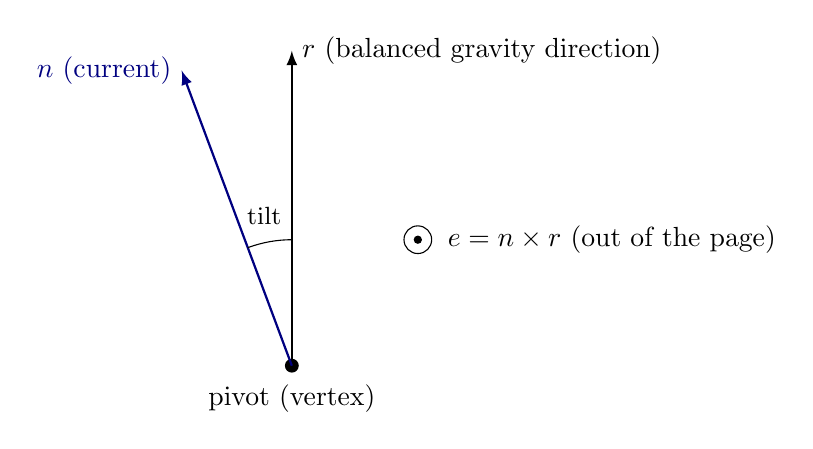
\begin{tikzpicture}[>=latex, thick]
    \fill (0,0) circle (2.5pt) node[below=3pt] {pivot (vertex)};
    \draw[->] (0,0) -- (0,4) node[right] {$\vect{r}$ (balanced gravity direction)};
    \draw[->, NavyBlue] (0,0) -- (-1.4,3.75) node[left] {$\vect{n}$ (current)};
    \draw[thin] (0,1.6) arc (90:110.5:1.6);
    \node at (-0.35,1.9) {\small tilt};
    \draw[thin] (1.6,1.6) circle (5pt);
    \fill (1.6,1.6) circle (1.5pt);
    \node[right] at (1.85,1.6) {$\vect{e} = \vect{n}\times\vect{r}$ (out of the page)};
  \end{tikzpicture}
  \caption{Tilt error at the vertex: $\vect{r}$ is the gravity direction in the calibrated
    balance position, $\vect{n}$ the current one, both measured in the body frame. Their cross
    product is the rotation vector of the tilt.}
  \label{fig:vertex_vectors}
\end{figure}

\section{Angular momentum about the vertical axis}
\label{sec:yaw_physics}

The wheels store angular momentum $\vect{h}$. Its tilt part is controlled exactly like the wheel
speed on the edge: gravity can remove it if the cube leans slightly. Its yaw part, however, cannot
be removed by gravity. If the controller fed back the yaw momentum in the same way as the tilt
momentum, it would form a positive feedback loop: more yaw momentum would cause a larger command
along the yaw axis, which would accelerate the wheels further. This effect was observed on the
real cube (\cref{sec:history}): with a negative yaw gain the yaw momentum grew exponentially with a
time constant of about \SI{2.4}{s} until the motors saturated, and the cube was visibly rotating
about its vertical axis.

The vertex controller therefore uses separate gains for the yaw part: a damping term on the yaw
rate and a term that slowly reduces the yaw momentum of the wheels. The reaction is transferred
to the ground through the friction at the pivot.

\section{Sensing the orientation}

The orientation is measured with an IMU that contains a three-axis accelerometer and a three-axis
gyroscope:
\begin{itemize}
  \item The \textbf{accelerometer} measures the gravity direction, which directly gives the tilt.
        However, it also measures every linear acceleration of the sensor. Each time the wheels
        accelerate, the cube jerks slightly, and the measured direction is disturbed.
  \item The \textbf{gyroscope} measures the angular rate. It is fast and not disturbed by linear
        accelerations, but integrating it to get an angle accumulates a slowly growing error
        (drift).
\end{itemize}
A \emph{complementary filter} combines both: the gyroscope is integrated for fast changes, and the
accelerometer slowly corrects the drift. With a filter constant $\alpha$ close to 1,
\begin{equation}
  \hat\theta_k = \alpha\left(\hat\theta_{k-1} + \omega\,\Delta t\right) + (1-\alpha)\,\theta_\text{acc} .
  \label{eq:cf}
\end{equation}
The firmware uses this filter on the edge and a three-dimensional version of it on the vertex
(\cref{sec:sensor_processing}).
